\documentclass[a4paper]{scrartcl}

\usepackage[
    fancytheorems, 
    fancyproofs, 
    noindent, 
]{adam}
\usepackage{floatrow}
\usepackage{import}
\usepackage{xifthen}
\usepackage{pdfpages}
\usepackage{transparent}
\usepackage{tikz}
\newcommand{\incfig}[2]{%
    \def\svgwidth{#1mm}
    \import{./figures/}{#2.pdf_tex}
}

\title{IB Optimisation}
\author{Martin von Hodenberg (\texttt{mjv43@cam.ac.uk})}
\date{\today}
\setcounter{section}{-1}

\allowdisplaybreaks

\begin{document}

\maketitle

These are my notes for the IB course Optimisation, which was lectured in Lent 2022 at Cambridge by Dr V.Jog. These notes are written in \LaTeX  \ for my own revision purposes. Any suggestions or feedback is welcome.

\tableofcontents
\newpage 

\section{Introduction}

The course is roughly divided into four parts:
\begin{enumerate}
	\item Convex optimisation (Lectures 1-3)
	\item Lagrange method (Lectures 4-5)
	\item Linear programming (Lectures 6-8)
	\item Applications of linear programming (Lectures 9-12)
\end{enumerate}

\begin{definition}[Optimisation problem]
	The basic structure of an optimisation problem is as follows:\\
	minimise $f(x)$ for $x \in X$, where in this course we take $X \subset \mathbb{R}^n$. The problem can have 'constraints' $h(x)=b$, where $h:\mathbb{R}^n \to \mathbb{R}^m$. We will look at minimising functions WLOG.
	
	\begin{enumerate}
		\item $f$ is called the objective function.
		\item The components of $x$ are called decision variables.
		\item $h(x)=b$ is called a functional constraint.
		\item $x \in X$ is called a regional constraint.
		\item $\{x: x \in X\}$ is called the feasible set $X (b) $.
		\item Problem is feasible if $X(b)\neq \emptyset$, and bounded if the minimum on $X(b)$ is bounded.
		\item A point $x^* \in X(b)$ is optimal if it minimises f over $X(b)$. The value $f(x^*)$ is called the optimal set. 
	\end{enumerate}
	
\end{definition}
\section{Convex optimisation} 
\subsection{Convexity}
\begin{definition}
	 A set $S \in \mathbb{R}^{n} $ is \vocab{convex} if for all $x,y \in S$, and all $\lambda \in [0,1]$, $(1-\lambda)x+\lambda y \in S$. (The line segment joining $x$ and $y$ lies in $S$.)  
	 \begin{figure}[H]
		\centering
		\incfig{70}{convex-drawing}
		\caption{Two subsets of $\mathbb{R}^{2} $: the left one is convex but the right one is not.}
	\end{figure}
\end{definition}
\newpage 

\begin{definition}
	 A function $f:S \rightarrow \mathbb{R}$ is \vocab{convex} if $S$ is convex, and for all $x,y \in S$, and $\lambda \in [0,1]$ , we have 
	 \[f((1-\lambda)x+\lambda y)\leq (1-\lambda)f(x)+ \lambda f(y).\] 
	 Intuitively, all the tangent lines to the function are below the function.We define $f$ to be concave if $-f$ is convex.
	 \begin{figure}[H]
		\centering
		\incfig{70}{convex-function-drawing}
		\caption{A convex function in $\mathbb{R}^2$.}
	\end{figure}
\end{definition}
\begin{remark}
	Linear functions are always both convex and concave, since we get equality in the above equation.
\end{remark}

\subsection{Unconstrained optimisation}
We want to find $\min f(x)$ where $f: \mathbb{R}^{n} \rightarrow \mathbb{R}$ is a convex function. This is a particularly simple case of optimisation, since convex functions have the important property that \emph{local information extends globally}. We will now look at a couple of ways to prove convexity, called the first- and second-order conditions.

\subsubsection{First order conditions for convexity}
Intuitively, for a convex function $f:\mathbb{R} \rightarrow \mathbb{R}$, we know that all the tangent lines to the function are below the function (see Figure 2). We can express this as 
\[f(y) \geq f(x)+(y-x)f'(x).\]
We can generalise this to higher dimensions:

\begin{theorem}[First-order conditions]
	 A differentiable $f:\mathbb{R}^n\rightarrow \mathbb{R}$ is convex iff for $x,y \in \mathbb{R}^{n} $ , we have 
	 \[f(y) \geq f(x)+\nabla f(x)^T (y-x).\]  
\end{theorem}

\begin{remark}
	If $\nabla f(x)=0$, then $f(y)\geq f(x) \implies$ $x$ minimises $f$.
\end{remark}

\begin{proof}
	\textbf{Convexity of $f \implies$ F-O conditions hold:}\newline 
	 Let $n=1$. For $x,y\in \mathbb{R}^{n}$, $t \in [0,1]$ we have 
	 \[f((1-t)x+ty)=f(x+t(y-x))\leq (1-t)f(x)+tf(y).\]
	 Therefore 
	 \[f(y) \geq f(x)+\frac{f(x+t(y-x))-f(x)}{t}.\] 
	 Taking $t \rightarrow 0$ , we conclude 
	 \[f(y) \geq f(x)+f'(x)(y-x).\]
	 For the general case, define a function $g(t)=f((1-t)x+ty)$, i.e $g: [0,1] \rightarrow \mathbb{R}$. Since $f$ is convex, $g$ is also convex. We can calculate 
	 \[g'(t)=\nabla f((1-t)x+ty)^T(y-x).\] 
	 Since $g$ is convex, by the above argument for $n=1$, we have $g(1)\geq g(0)+g'(0)(1-0)$. 
	 \[\implies f(y) \geq f(x)+\nabla f(x)^T(y-x).\] 
	 \textbf{F-O conditions hold $\implies$ convexity:}\\
	 Define $x_t=(1-t)x+ty$. We have the two equations
	 \begin{align}
		 f(x) &\geq f(x_t)+\nabla f(x_t)^T (x-x_t)\\
		 f(y) &\geq f(x_t)+\nabla f(x_t)^T (y-x_t)
	 \end{align}
	 Now we add $(1-t)\times$ equation (1) to $t \times$ equation 2. Noting that $x-x_t=tx-ty$ and $y-x_t=(1-t)y-(1-t)x$, we get 
	 \[(1-t)f(x)+tf(y)\geq f(x_t)+\nabla f(x_t)^T (0).\] 
	 This concludes the proof.
\end{proof}

\subsubsection{Second-order conditions for convexity}

Next we look at second-order conditions. In one dimension, we would expect that $f'$ being increasing, i.e $f''(x) \geq 0$, would give us convexity. We generalise this to $n$ dimensions using the Hessian matrix, which we saw in IA Differential Equations. It has entries $[\nabla^2f(x)]_{ij}=\frac{\partial^2 f(x)}{\partial x_i x_j} $.

\begin{definition}[Semidefinite matrix]
	 A matrix $A$ is called \vocab{positive semidefinite} if for all $ x \in \mathbb{R}^{n} $ we have $x^T Ax \geq  0$. Equivalently, all eigenvalues of $A$ are non-negative. 
\end{definition}

\begin{remark}
	The Taylor expansion in $n$ dimensions is 
	\[f(y)=f(x)+\nabla f(x)^T(y-x)+\frac{1}{2} (y-x)^T \nabla^2 f(x)(y-x)+\ldots.\] 
\end{remark}

\begin{theorem}[Second-order condition]
	 A twice differentiable $f: \mathbb{R}^{n}\rightarrow \mathbb{R}$ is convex if $\nabla^2 f(x)$ is positive semidefinite, i.e $x^T\nabla^2 f(z) x\geq 0$ for all $ x,z \in \mathbb{R}^{n}$.  
\end{theorem}

\begin{proof}
	 Using the Taylor expansion of $f$ we have 
	 \[f(y)=f(x)+\nabla f(x)^T(y-x) + \frac{1}{2} (y-x)^T \nabla^2 f(z)(y-x).\]
	 where $z=(1-\lambda)x+ \lambda y$ for some $\lambda\in [0,1]$. (IA Analysis).\\
	 We have $f(y) \geq f(x)+\nabla f(x)^T(y-x)$. Then by the first-order condition theorem, $f$ is convex. 
\end{proof}

\subsection{The gradient descent algorithm}
Recall we have an unconstrained optimisation problem: 
\[\text{minimise }  f(x), f:\mathbb{R}^{n} \rightarrow \mathbb{R} \text{ is a convex function} .\] 
In order to solve this, we could apply agree a 'greedy method' where we pick an initial point $x_0$ and iteratively pick points $x_1,x_2,\ldots$ near this point so that the gradient of $f$ at $x_n$ is decreasing. In which direction should we decrease $x_n$? Note that by Taylor's expansion, with small $\epsilon>0$, 
\[f(x-\epsilon \nabla f(x))\approx f(x)-\epsilon \nabla f(x)^T \dot \nabla f(x)=f(x)-\epsilon ||f(x)||^2 \leq f(x).\]

We call the direction $-\nabla f(x)$ the descending direction. (Note we could also choose any other direction $v$ so that $f(x)^T \dot v <0$.) We now formalise this process in an algorithm.

\begin{definition}[Gradient descent method]
	Define an algorithm:
	 \begin{enumerate}
		 \item Start at some point $x_0$. Set $t=0$.
		 \item Repeat the following: 
		 \begin{itemize}
			 \item Find a descending direction $v_t$ (e.g $-\nabla f(x_t)$)
			 \item Choose a step size $\eta_t$ (can depend on $t$)
			 \item Update $x_{t+1}=x_t+\eta_t v_t$
		 \end{itemize}
		 \item Stop when some criterion is met (e.g $\nabla f(x_t)=0$, $t$ is large enough)
	 \end{enumerate}
\end{definition}

For the scope of this course, we need to make assumptions about our convex function.
\subsubsection{Smoothness assumption}

\begin{definition}[Smoothness assumption]
	 We say that a continuously differentiable function $f: \mathbb{R} \rightarrow \mathbb{R}$ is $\beta$-smooth or $\beta$-Lipschitz if 
	 \[||\nabla f(x)-\nabla f(y)|| \leq \beta ||x-y||.\] 
	 Those who have taken IB Analysis and Topology will be familiar with this concept.
\end{definition}
\begin{remark}
	If $f$ is twice-differentiable, then $\beta$-smoothness implies that $\nabla^2 f(x)\leq \beta I$. Equivalently, all eigenvalues of $\nabla^2 f(x)$ are $\leq \beta$. $\beta$-smoothness can be summed up by the fact that \emph{the linear approximation is close to $f$ in a small neighbourhood around $x$}.
\end{remark}

\begin{proposition}
	If $f$ is $\beta$-smooth and convex, then 
	\[f(x)+\nabla f(x)^T(y-x) \leq f(y) \leq f(x)+\nabla f(x)^T(y-x)+ \frac{\beta}{2}||x-y||^2.\]
\end{proposition}

\begin{proof}
	 The left-hand inequality follows by convexity.\newline 
	 For the right hand inequality, by Taylor's theorem,
	 \begin{equation*}
		  \begin{split}
			  f(y)=&\nabla f(x)^T(y-x)+\frac{1}{2}(y-x)^T \nabla^2 f(z)(y-x)\\
			  &\leq f (x) +\nabla f (x)^T (y-x) + \frac{1}{2} (y-x)^T (\beta I)(y-x)\\
			  &=f(x)+\nabla f (x)^T (y-x) + \frac{\beta}{2} ||x-y||^2
		  \end{split}
	 \end{equation*}
\end{proof}

\begin{corollary}
	At any point $x$,
	\[f(x-\frac{1}{\beta}\nabla f (x))\leq f(x)-\frac{1}{2\beta}||f(x)||^2.\]
\end{corollary}
\begin{proof}
	 Let's look at 
	 \[f(x)+\nabla f(x)^T (y-x)+\frac{\beta}{2}||x-y||^2,\]
	 and try to minimise it over $y$ for a fixed $x$.
	 \[\nabla y (f (x)^T (y-x) + \frac{\beta}{2}||x-y||^2)=\nabla f(x)-\beta (x-y)=0.\]
	 \[\implies \nabla \frac{\nabla f (x)}{\beta}=x-y \implies y=x- \frac{1}{\beta}\nabla f	(x).\]
	 Plug this value of $y$ into the above claim: 
	 \begin{equation*}
		  \begin{split}
			f(x-\frac{1}{\beta}\nabla f(x))&\leq f(x)+\nabla f(x)^T (\frac{-1}{\beta}\nabla f(x))+\frac{\beta}{2}||\frac{1}{\beta}\nabla f(x)||^2\\
			&=f(x)-\frac{1}{\beta}||\nabla f(x)||^2+\frac{1}{2\beta}||\nabla f(x)||^2\\
			&=f(x)-\frac{1}{2\beta}||\nabla f(x)||^2
		  \end{split}
	 \end{equation*}	
\end{proof}

\begin{corollary}[Improved first-order condition]
	
	\[f(y)\geq f(x)+\nabla f (x)^T(y-x)+\frac{1}{2\beta}||\nabla f(x)-\nabla f (y)||^2.\]
	
\end{corollary}
\begin{proof}
	 For any $z$, we have 
	 \[f (x)+\nabla f (x)^T (z-x)\leq f (z)\leq f(y)+\nabla f (y)^T (z-y)+\frac{\beta}{2}||z-y||^2.\]
	 This implies 
	 \[f (x)-f (y)\leq \nabla f (x)^T (x-z)+\nabla f (y)^T (z-y)+\frac{\beta}{2}||z-y||^2.\]
	 To minimise the RHS, set $\nabla_z=0$. We get $-\nabla f (x)+\nabla f (y)+\beta (z-y)=0$, which implies 
	 \[z=\frac{f (x)-f (y)}{\beta}+y.\]
	 Subbing into the RHS, we get 
	 \[f (x)- f (y)\leq \nabla f (x)^T (x-y)-\frac{1}{2\beta}||\nabla f (x)-\nabla f (y)||^2.\]
\end{proof}
\subsubsection{Strong convexity assumption}
We now introduce a new type of convexity we assume. In essence, it tells us that \emph{if the gradient is small, we are close to the optimum}.
\begin{definition}[Strong convexity assumption]
	 A function $f: \mathbb{R}^{n} \to \mathbb{R} $ is $\alpha$-strongly convex if 
	 \[f(y)\geq f (x)+ \nabla f (x)^T (y-x)+\frac{\alpha}{2}||x-y||^2.\]
	 If $f$ is twice differentiable, then 
	 \[\nabla^2 f (x)\geq \alpha I \ \forall x.\]
\end{definition}

\begin{proposition}
	Let $f$ be $\alpha$-strongly convex. Let $p^*$ be the optimal cost. Then for any $x$ we have \[p^* \geq f(x)-\frac{1}{2\alpha}||\nabla f(x)||^2.\]
\end{proposition}
\begin{remark}
	If $||\nabla f (x)||\leq \sqrt{2\alpha \epsilon}$ then $p^* \geq f(x)-\epsilon$, i.e 
	\[p^* \leq f (x) \leq p^*+ \epsilon.\]
	
\end{remark}
\begin{proof}
	 The $\alpha$-strong convexity assumption gives us 
	 \[\min_y f(y)\geq \min_y f (x)+ \nabla f (x)^T (y-x)+\frac{\alpha}{2}||x-y||^2.\]
	 Setting $\nabla_y$ of the RHS=0, we get $y=x-\frac{\nabla f (x)}{\alpha}.$\newline 
	 Plugging this value of $y$ in the RHS, we get 
	 \[f(x)+\nabla f(x)^T (\frac{-\nabla f (x)}{\alpha})+\frac{\alpha}{2}||\frac{\nabla f(x)}{\alpha}||^2=f (x)- \frac{1}{2\alpha}||\nabla f (x)||^2.\]
	 
\end{proof}

We might also want to ask: how close is the true optimiser $x^*$ to our current point $x$? It turns out $\alpha$-strong convexity gives us an answer to this too.

\begin{proposition}
	Let $x \in S$, and $x^*$ be the true optimiser. Then
	\[||x-x^*||\leq \frac{2}{\alpha}||\nabla f (x)||.\]
	
\end{proposition}
\begin{proof}
	 \begin{equation*}
		  \begin{split}
			  f(x^*)&\geq f(x)+\nabla f(x)(x^*-x)+ \frac{\alpha}{2}||x-x^*||^2\\
			  &\geq f(x)-||\nabla f(x)||||x^*-x||+\frac{\alpha}{2}||x-x^*||^2 \text{ by Cauchy-Schwartz} 
		  \end{split}
	 \end{equation*}
	We already know that $f (x^*)\leq f (x)$. Therefore 
	\[0 \geq f (x^*)-f (x)\geq -||\nabla f (x)|| \ ||x^*-x||+ \frac{\alpha}{2}||x-x^*||^2.\]
	So $||\nabla f (x)||\ ||x-x^*||\leq \frac{2}{\alpha}||\nabla f (x)||^2$, and thus 
	\[||x-x^*||\leq \frac{2}{\alpha}||\nabla f (x)||.\]
	
\end{proof}
\subsubsection{Efficiency of gradient descent}

\begin{theorem}
	Gradient descent with step size $\frac{1}{\beta}$ satisfies: 
	\[f(x_t)-f(x^*)\leq (1-\frac{\alpha}{\beta})^t (f(x_0)-f(x^*))\leq e^{\frac{-\alpha t}{\beta}} (f (x_0)- f (x^*))\leq e^{\frac{-\alpha t}{\beta}} \frac{\beta}{2}||x^*-x_0||^2.\]
	Note this is very efficient; the error decreases exponentially!

\end{theorem}
\begin{proof}
	 \begin{equation*}
		  \begin{split}
			  f(x_{t+1})-f (x*)&\leq f (x_t)- f (x^*)-\frac{1}{2\beta}||\nabla f(x_t||^2\\
			  &\leq f(x_t)- f (x^*) - \frac{\alpha}{\beta}(f (x_t)-f (x^*)) \text{ by strong convexity} \\
			  &\leq (1-\frac{\alpha}{\beta}	)(f (x_t)-f (x^*))
		  \end{split}
	 \end{equation*}
	 Using induction, conclude that 
	 \[f (x_t)-f (x^*)\leq (1-\frac{\alpha}{\beta})^t (f (x_0)-f (x^*)).\]
	 Because $f$ is $\beta$-smooth, we have 
	 \[f(x_0)\leq f (x^*)+\underbrace{\nabla f (x)^t (x_0-x^*)}_{=0}+\frac{\beta}{2}||x_0-x^*||^2.\]
\end{proof}
\begin{remark}
	With this algorithm, the number of steps needed to ensure error $\leq \epsilon$ is 
	\[\frac{\beta}{\alpha}\log (\frac{f (x_0)-f (x^*)}{\epsilon} ).\]
	The $\log (\frac{1}{\epsilon })$ dependence is called 'linear convergence'.
	
\end{remark}
\subsection{Alternatives to gradient descent}
\subsubsection{Newton's method}
When we use gradient descent, the factor $(1-\frac{\alpha}{\beta})$ controls the speed of convergence. We call $\frac{\beta}{\alpha}$ the \vocab{condition number} of $f$ (note we always have $\beta>\alpha$). If the condition number is large, then convergence will be slow and we may want to consider other algorithms. Let's look at an example:

\begin{example}
	Let $f: \mathbb{R}^{2} \to \mathbb{R} $ be given by 
	\[f(x,y)=\frac{1}{2}(x^2+100y^2).\]
	Now we have 
	\[\nabla^2 f (x,y)=\begin{pmatrix}
	1&0\\0&100
	\end{pmatrix}
	.\]
	Note that $I\leq \nabla^2 f (x,y)\leq 100I$. Our condition number is 100, which is very large! The contours of $f$ are very stretched ellipses in $\mathbb{R}^2$. If we use gradient descent on a point, it will comparatively overshoot a very large amount in the $y$ direction. Therefore convergence will be slow.
	\begin{figure}[H]
		\centering
		\incfig{70}{ellipse-contours}
		\caption{The path oscillates as it overshoots each time in the $y$ direction.}
	\end{figure}
\end{example}
We need another method in these cases. This is given by Newton's method:
\begin{definition}[Newton's method]
	 Here we use a modified version of gradient descent, with 
	 \[x_{t+1}=x_t-(\nabla^2 f (x))^{-1}\nabla f (x_t).\]
	 The derivation of this comes from the second order Taylor approximation of $f$ at $x_t$: 
	 \[f(x)\approx f (x_t)^T (x-x_t)+\frac{1}{2}(x-x_t)^T \nabla^2 f (x_t)(x-x_t).\]
	 If we minimise the RHS wrt. $x$, then we get $x=x_t-(\nabla^2 f(x))^{-1}\nabla f (x)$. This method of minimising the second-order approximation is shown in the figure below:
	 \begin{figure}[H]
		\centering
		\incfig{70}{newton-curve}
		\caption{The second-order approximation, shown in red, is repeatedly minimised as we increment $t$.}
	\end{figure}
	 
\end{definition}
\begin{remark}
	Intuitively, Newton's method is excellent for functions with accurate second-order approximations.
\end{remark}
\subsubsection{Convergence of Newton's method}
We will not do the analysis in this course, but Newton's method satisfies 
\[||x_{t+1}-x^*||\leq C ||x_t-x^*||^2 \text{, as long as } x_t \text{ is close enough to } x^*.\]
In one dimension, Newton's method is a root-finding algorithm:\newline 
Take $f: \mathbb{R} \to \mathbb{R}$, and let $f'=g$. Write 
\[x_{t+1}=x_t-\frac{f'(x_t)}{f'' (x_t)}=x_t-\frac{g (x_t)}{g' (x_t)}.\]
If we set $f'(x_{t+1})=g (x_{t+1})=0$, i.e looking for a stationary point of $f$ (which is the same as a root of $g$ if $g$ is convex) then we can write $g (x_{t+1})\approx g (x_{t})+g' (x_t)(x_{t+1}-x_t)=0$, and this gives the previous equation as expected. The root-finding algorithm is illustrated below:
\begin{figure}[H]
	\centering
	\incfig{70}{newton-root}
	\caption{Newton's method applied in one dimension as a root-finding algorithm. Note the speed of convergence displayed.}
\end{figure}
\subsubsection{Barrier methods}
What if the function we had to minimise involved constraints? We can write the optimisation problem as 
\[\text{minimise } f (x) \text{subject to} f_i (x)\leq 0 \ \forall 1 \leq i \leq n .\]
The way we approach this is to transform the constrained problem into an unconstrained one. The way we do this is by defining some new functions for the new optimisation problem:
\begin{equation*}
	 \text{minimise } f (x)+\sum_{i=1}^{n}\phi (f_i (x)), \phi= \begin{cases}
		 \infty & f_i (x)>0 \text{ for any } 1 \leq i \leq m\\
		 0 & f_i (x)\leq 0\text{ for all } 1 \leq i \leq m  
	 \end{cases}
\end{equation*}

This may still be difficult to deal with, so we can define a \vocab{logarithmic barrier function}: 
\[\text{minimise } tf (x) - \sum \log (-f_i (x)).\]
Here we are taking $\phi (x)=-\log (-x)$, so we are using an approximation: however we can make this negligible in practice by choosing suitable $t$.

\begin{definition}[Barrier method]
	We define an algorithm:
	 \begin{enumerate}
		\item Find a point $x$ in the feasible set. Set $t>0$.
		\item Repeat: 
		\begin{itemize}
			\item Solve $\min t f (x)+\sum_{i=1}^{n}\phi (f_i (x))$ with $x$ as the starting point, use Newton's method.
			\item Set $x=x^* (t)$.
			\item Stop if $t$ is large enough
			\item Increase $t=\alpha t$ for $\alpha>1$.
		\end{itemize}
	 \end{enumerate}
\end{definition}

\section{The Lagrange multiplier method}
Suppose we want to minimise $f(x)$ for $x \in X$ subject to constraints $h(x)=b$ where $h: \mathbb{R}^{n} \to \mathbb{R}^m $.\newline 
The \vocab{Lagrangian} associated with this problem is 
\[L (x, \lambda)=f (x)-\lambda^T (h (x)-b).\]
Note that $\lambda \in \mathbb{R}^{m} $.
We want to minimise $L (x, \lambda)$ over $x \in X$ for some value of $\lambda$.
\subsection{Lagrange sufficiency}

\begin{theorem}[Lagrange sufficiency theorem]
	 Suppose we can find a $\lambda^*$ such that:
	 \begin{enumerate}
		\item $\min_{x \in X} L (x,\lambda^*)=L (x^*,\lambda^*)$ for some $x^* \in X$.
		\item $x^* \in X(b)=\{x: x \in X, h(x)=b\}$, the feasible set for our constrained problem.
	 \end{enumerate}
	 Then $x^*$ is optimal for 1, i.e $\min_{x \in X(b)}f (x)=f (x*)$.
	 
\end{theorem}
\begin{proof}
	 Condition 2 says that $f (x^*)\geq \min_{x \in X(b)}f (x)$ because $x^*$ is feasible. We have 
	 \begin{equation*}
		  \begin{split}
			\min_{x \in X(b)}f (x)&=\min_{x \in X(b)}f (x)-(\lambda^*)^T (h (x)-b)\\
			&\geq \min_{x \in X}f (x)-(\lambda^*)^T (h (x)-b)\\
			&=L (x^*,\lambda^*)\\
			&=f(x^*)-(\lambda^*)^T (h (x^*)-b)\\
			&=f (x^*).
		  \end{split}
	 \end{equation*}
	 
\end{proof}
Let's look at an example.
\begin{example}
	Minimise $-x_1-x_2 +x_3 $ subject to $x_1^2+x_2^2=4, x_1 +x_2 +x_3 =1$. Here we have 
	\[h(x_1,x_2,x_3)=\begin{pmatrix}
	x_1^2+x_2^2 \\x_1 +x_2 +x_3
	\end{pmatrix}
	,b=\begin{pmatrix}
	4\\1
	\end{pmatrix}
	 .\]
	Our Lagrangian is 
	\[L(x,\lambda)=(-x_1-x_2+x_3)-\lambda_1(x_1^2+x_2^2-4)-\lambda_2(x_1 +x_2 +x_3 -1).\]
	We can rewrite this as 
	\[L(x,\lambda)=(-(1+\lambda_2)x_1-\lambda_1 x_1^2)= (-(1+\lambda_2)x_2-\lambda_1 x_2^2)+(1-\lambda_2)x_3 + (4\lambda_1+\lambda_2).\]
	Now fix $\lambda$, and try to find $\min_{x \in \mathbb{R}^{n} }L(x,\lambda)$. We'll only be interested in $(\lambda_1,\lambda_2)$ so that the minimum is finite.
	\begin{itemize}
		\item If $\lambda_1>0$, the infinimum is $-\infty$.
		\item If $\lambda_2\neq 1$, the infinimum is $-\infty$.
	\end{itemize}
	Let's look at $\lambda_1\leq 0, \lambda_2=1$.
	\[\frac{d}{dx_1}(-(1+\lambda_2)x_1-\lambda_1 x_1^2)=-(1+\lambda_2)-2\lambda_1 x_1=0 \implies x_1=\frac{-1}{\lambda_1}.\]
	Similarly, differentiating wrt. $x_2$ gives $x_2=\frac{-1}{\lambda_1}$. Can we pick $\lambda_1$ so that $(x_1,x_2)$ satisfy the constraints? We need 
	$x_1^2+x_2^2=4, x_1 +x_2 +x_3 =1$. Therefore 
	\[x_1^2=x_2^2=2 \implies x_1=x_2=\sqrt{2}.\] 
	Since $\lambda_1 \leq 0$, our optimiser is 
	\[x=(\sqrt{2},\sqrt{2},1-2 \sqrt{2}).\]
\end{example}

Let's formalize the above method for solving 
\[\min_{x \in X} f(x) \text{ with }  h (x)\leq b.\]
\begin{enumerate}
	\item Add a slack variable $s$ to transform the problem into
	\[\min_{x \in X} f(x) \text{ with } h (x)+s=b, s \geq 0.\]
	\item Set $L (x,\lambda,s)=f(x)-\lambda^T (h(x)+s-b)$, and let 
	\[\Lambda=\{\lambda: \inf_{x \in X, x \geq 0} L(x,\lambda,s)\geq -\infty\}.\]
	\item For each $\lambda \in \Lambda$, find $x^*(\lambda)$,$s^*(\lambda)$ such that 
	\[\min_{x \in X, s \geq 0}L(x,\lambda,s)=L(x^*(\lambda),\lambda,s^*(\lambda)).\]
	\item Find a $\lambda^* \in \Lambda$ such that $(x^* (\lambda^*), s^* (\lambda^*))$ is feasible; i.e $h (x^* (\lambda^*))=b$ and $s^* (\lambda^*)\geq 0$.
\end{enumerate}
\subsection{Complementary slackness}
Let's suppose we want to minimise $f(x)-\lambda^T (h(x)+s-b)$ subject to $ x \in X, s \geq 0$. Suppose for $\lambda \in \Lambda$, we solve to arrive at $x^*(\lambda), s^*(\lambda)$. Note we must have all the components $\lambda_i\leq 0$ in order to keep $\lambda \in \Lambda$. We have 
\[-\lambda^T s=-\sum \lambda_i s_i=\sum_{i=1}^{m}(\lambda_i)\dot s_i.\]
$\min -\lambda^T s =0$, which means $\lambda_i s_i=0 \ \forall 1 \leq i \leq m$.
Consider our inequalities $h_i(x)+s_i=b_i$. If any of these inequalities are not equalities, then for that $i$ we must have $\lambda_i=0$. This is called \vocab{complementary slackness}.

\begin{example}
	Problem: 
	\[\min x_1-3x_2 \text{ subject to } x_1^2+x_2^2 \leq 4,  x_1+x_2 \leq 2.\]
	Let's apply our algorithm.
	\begin{enumerate}
		\item Add slack variables: our problem is now \[\min x_1-3x_2 \text{ subject to } x_1^2+x_2^2+s_1= 4,  x_1+x_2+s_2= 2, s_1,s_2 \geq 0.\]
		\item Work out 
		\[L(x,\lambda,s)=((1-\lambda_2)x_1-\lambda_1 x_1^2)+((-3 -\lambda_2)x_2-\lambda_1x_2^2)-\lambda_1s_1-\lambda_2s_2+(4 \lambda_1+2 \lambda_2).\]
		\item We must have $\lambda_1,\lambda_2\leq 0$ by complementary slackness. At the optimum, $\lambda_1s_1=\lambda_2 s_2=0$. By differentiating $L$, we get the system of equations 
		\begin{align*}
			(1-\lambda_2)-2 \lambda_1 x_1 &=0.\\
			-3-\lambda_2-2\lambda_1 x_2 &=0.
		\end{align*}
		These show we can't have $\lambda_1=0$ and thus $\lambda_1 <0$ and $s_1=0$. There are two more cases:
		\begin{itemize}
			\item If $\lambda_2<0$, then $s_2=0$. We have the two equations above, and then by complementary slackness we also know that 
			\[x_1^2+x_2^2=4, x_1+x_2=2.\]
			Solving these gives $(x_1,x_2)=(0,2)$ or $(2,0)$. But with both of these solutions the first two equations give one of the $\lambda_i >0$. So we don't have any solutions in this case.
			\item The last case is $\lambda_1<0,\lambda_2=0,s_1=0$. Here we get the two equations above and $x_1^2+x_2^2=4$. Here we get 
			\[x_1=\frac{1}{2\lambda_1}, x_2=\frac{-3}{2\lambda_1}.\]
			Therefore $\lambda_1^2=\frac{5}{8}$ and thus 
			\[(x_1,x_2)=(-\sqrt{\frac{2}{5}},3 \sqrt{\frac{2}{5}}).\]
			So we are done by Lagrange sufficiency.
		\end{itemize}
	\end{enumerate}
\end{example}
\subsection{Strong duality and shadow prices}
For some optimisation problems that we solve using the Lagrange method, for \emph{every} $\lambda$ we can find a feasible $x^*$ such that 
\[\min_{x \in X} L (x, \lambda)=L(x^*,\lambda).\]
This property of an optimisation problem is called \vocab{strong duality}.
Before we do this, however, let's start with a weaker theorem.
\begin{theorem}[Weak duality]
	 For a Lagrange problem define 
	 \[g (\lambda)=\inf_{x \in X}L (x,\lambda).\]
	 If $x \in X (b)$, and $\lambda \in \Lambda$, then $f (x)\geq g (x)$. In particular,
	 \[\inf_{x \in X(b)}f(x) \geq \sup_{\lambda \in \Lambda}g (\lambda).\]
\end{theorem}
\begin{proof}
	For all $\lambda \in \Lambda$,
	 \begin{equation*}
		  \begin{split}
			\inf_{x \in X(b)}f(x)&=\inf_{x \in X(b)}(f(x)- \lambda^T (h(x)-b))\\
			&\geq \inf_{x \in X}(f(x)- \lambda^T (h(x)-b))\\
			&=\inf_{x \in X}L (x,\lambda)\\
			&=g (\lambda).
		  \end{split}
	 \end{equation*}
	 
\end{proof}

The problem of maximising $g (\lambda)$ subject to $\lambda \in \Lambda$ is called the \vocab{dual problem}, and the problem of minimising $f (\lambda)$ subject to $x \in X(b)$ is called the \vocab{primal problem}.\newline 
The \vocab{duality gap} is 
\[\inf_{x \in X(b)}f(x)- \sup_{\lambda \in \Lambda}g (\lambda).\]
If the gap is 0, we say that \vocab{strong duality} holds.
\begin{definition}[Hyperplane]
	 A function $\phi: \mathbb{R}^{m} \to \mathbb{R} $ is said to have a supporting hyperplane at $b$ if there exists a $\lambda \in \mathbb{R}^{m}$ such that for all $c \in \mathbb{R}^{m} $, the following holds: 
	 \[\phi(c)\geq \phi (b)+ \lambda^T (c-b).\]
	 This is easy to visualise in one dimension: There exists a tangent to the curve $\phi$ at $(b,\phi(b))$ such that the tangent is below the curve.
	 \begin{figure}[H]
		\centering
		\incfig{70}{hyperplane-sketch}
		\caption{The hyperplane in one dimension is a tangent below the curve with slope $\lambda$.}
	\end{figure}
\end{definition}

\begin{definition}[Value function]
	 Define the \vocab{value function} $\phi: \mathbb{R}^{m} \to \mathbb{R} $ associated with the primal problem as follows: 
	 \[\phi (c)=\inf_{x \in X(c)}f(x).\]
\end{definition}

\begin{theorem}[Strong duality]
	 Strong duality holds if and only if the vlaue function $\phi$ has a separating hyperplane at $b$.
\end{theorem}
\begin{proof}
	 We prove both directions.\newline 
	 \textbf{Separating hyperplane $\implies $ strong duality:}\newline 
	 There exists $\lambda$ such that $\phi(c)\geq \phi (b)+ \lambda^T (c-b)$.
	 Then we have
	 \begin{equation*}
		  \begin{split}
			  g (\lambda)&=\inf_{x \in X}(f (x)- \lambda^T (h (x)-b))\\
			  &=\inf_{c}\inf_{x \in X}(f (x)- \lambda^T (h (x)-c)-\lambda^T (c-b))\\
			  &=\inf_{c}(\phi(c)-\lambda^T (c-b))\\
			  \geq \phi(b).
		  \end{split}
	 \end{equation*}
	 Weak duality gives $g (\lambda)\leq \phi (b)$, and so $g (\lambda)=\phi(b)$; i.e, strong duality holds.
	 \textbf{Strong duality holds $\implies $ separating hyperplane exists at $b$:}\newline 
	 There exists $\lambda$ such that $g (\lambda)=\phi (b)$.
	 \begin{equation*}
		\begin{split}
			\phi (b)=g (\lambda)&=inf_{x \in X} (f (x)-\lambda^T (h (x)-b))\\
			&=inf_{x \in X} (f (x)-\lambda^T (h (x)-c)-\lambda^T (c-b))\\
			&\leq \phi (c)- \lambda^T (c-b) \text{ by weak duality} 
		\end{split}
   \end{equation*}
	This means that $\lambda$ gives the supporting hyperplane at $b$.
\end{proof}

\subsubsection{When does $\phi (b)$ have a separating hyperplane?}
\begin{theorem}[Separating hyperplanes and convex functions]
	A function $\phi: \mathbb{R}^{n} \to \mathbb{R} $ is convex if and only if every point $b \in \mathbb{R}^{n} $ has a separating hyperplane.	\newline 
\end{theorem}
\begin{proof}
	We state this theorem without proof.
\end{proof}

\begin{theorem}[Convexity conditions]
	 Consider the problem of minimising $f (x)$ with $x \in X, h (x)\leq b$. Then $\phi$ is convex if: 
	 \begin{enumerate}
		 \item $X$ is convex
		 \item $f$ is convex
		 \item $h$ is convex
	 \end{enumerate}
\end{theorem}
\begin{proof}
	 This is left to be proved on Example Sheet 1.
\end{proof}
\subsubsection{Economics interpretations}
Let's say we have a factory owner. He makes $n$ types of products using $m$ types of raw materials (which have a finite supply). Let's say that with $x=(x_1,\ldots ,x_m)$ raw materials he makes a profit of $f (x)$.\newline 
Further, let $h_j (x)$ is the raw material consumed of type $j$. Our problem is to maximise $f (x)$ such that $h_i (x) \leq b_i$ for $1 \leq i \leq m$, and $x \geq 0.$\newline 
If $(\epsilon_1,\ldots , \epsilon_m)$ amount of raw material is offered to the factory owner, how much is it worth? For small enough $\epsilon $, we have 
\[\phi (b+\epsilon )-\phi (b)\approx \sum_{j=1}^{m}\frac{\partial \phi (b)}{\partial b_j} \epsilon_j.\]

The vector of prices $(\frac{\partial \phi (b)}{\partial b_1} ,\ldots , \frac{\partial \phi (b)}{\partial b_m} )=\nabla \phi (b)$. These are called "shadow prices".

\begin{theorem}
	 If $\phi$ is differentiable at $b$ and has a separating hyperplane given by $\lambda$, then $\lambda=\nabla \phi (b)$.
\end{theorem}
\begin{proof}
	 Let $a= (a_1,\ldots , a_m)$ be an arbitrary vector. Pick $\delta>0$.
	 \begin{equation*}
		  \begin{split}
			  \frac{\phi (b+\delta a)- \phi (b)}{\delta}&\geq \lambda^T a\\
			  \implies \nabla \phi (b)^T a &\geq \lambda^T a \text{ for every vector } a.\\
			  \implies \nabla \phi (b)&=\lambda.
		  \end{split}
	 \end{equation*} 
\end{proof}

The Lagrange multiplier at $b$ is the vector of partial derivatives, i.e the vector of shadow prices. The intutive interpretation of 'not wanting to pay any more' when you have enough of a certain raw material (that shadow price being 0) is an interpretation of complementary slackness.\newline \\
Now let's look at the dual problem. If the raw material seller charges a price $\lambda$, and the finished product is consumed when he sells it, then 
\[\lambda^T (h (x)-b)-f (x)\]
is the Lagrangian he is trying to minimise. But the factory producer is producing $x^*(\lambda)$ to maximise 
\[f(x)-\lambda^T (h (x)-b).\]
Let's call $g (\lambda)=\lambda^T (h (x^* (\lambda)-b)- f ( x^* (\lambda)))$. The seller is trying to maximise $g$. This provides a good example of the dual problem.

\section{Solving linear programs}
\begin{definition}[Linear program]
	 A general linear program is an optimisation problem of 
	 \begin{equation*}
		\text{minimise } c^Tx \text{, subject to }
		  \begin{cases}
			  a_i^T x \geq b_i& i \in M_1\\
			  a_i^T x \leq b_i& i \in M_2\\
			  a_i^T x = b_i& i \in M_3\\
			  x_j \geq 0& j \in N_1\\
			  x_j \geq 0& j \in N_2
		  \end{cases}
	 \end{equation*}
	 Two linear programs are equivalent if given a feasible solution for one formulation, we can construct a feasible solution for the other formulation with the same cost. The \vocab{general form} of a linear program is:
	 \[\text{minimise } c^T x \text{ subject to } Ax \geq b.\]
	 where 
	 \[A=\begin{pmatrix}
	 \ldots &A_1^T&\ldots \\
	 \ldots &A_2^T&\ldots \\
	  &\vdots&\\
	  \ldots &A_m^T&\ldots 
	 \end{pmatrix}, \ b = \begin{pmatrix}
	 b_1\\b_2\\\vdots\\b_m
	 \end{pmatrix}
	 .\]
	A linear problem is said to be in \vocab{standard form} if it has the form
	\[\text{minimise } c^T x \text{ subject to } Ax \geq b, x \geq 0.\]
	We can do this WLOG	since we can split $x$ into two vectors $x^{+}-x^{-}$ such that each of their entries are positive and then minimise $c^T(x^{+}-x^{-})$ with the respective modified version of $A$.
\end{definition}

\subsection{Maximising convex functions}
Recall that $\min c^Tx= \max -c^Tx $. So solving linear programs is a special case of maximising convex functions. Let's consider the general problem for a convex set $C$:
\[\text{maximise } f (x) \text{ subject to } x \in C.\]
Take $z=(1-\lambda)x +\lambda y $ where $x,y \in C.$ We have 
\[f (z)\leq (1-\lambda)f (x)+\lambda f (y) \leq \max \{f (x), f (y)\}.\]
This is true for all $x,y \in C$, so the global maximum must be maximised somewhere on the 'boundary' of $C$.
\begin{definition}[Extreme point]
	 A point $x$ in a convex set $C$ is an \vocab{extreme point} if it cannot be written as $(1-\delta)y+\delta z$ for $\delta \in (0,1)$ and $y,z$ distinct.
\end{definition}
\begin{remark}
	"Convex functions on convex sets are maximised at extreme points".
\end{remark}
\subsection{Basic solutions and basic feasible solutions}
Recall our linear problem: \newline 
minimise $c^Tx$ such that $Ax=b, x \geq 0$ with $A \in L(\mathbb{R}^{n},\mathbb{R}^{m} ), x \in \mathbb{R}^{n} , b \in \mathbb{R}^{m}$.\newline 
We make two assumptions:
\begin{itemize}
	\item[($\ast$)] All $m$ rows of $A$, $(a_1^T,\ldots ,a_m^T)$ are linearly independent.
	\item[($\ast\ast$)] Every set of $m$ columns of $A$ is linearly independent WLOG. We can see these first two assumptions as getting rid of redundant variables.
	\item[($\ast\ast\ast$)] Every basic solution has exactly $m$ non-zero entries. (Non-degeneracy assumption)
\end{itemize}
We can't make assumption $(\ast \ast \ast)$ WLOG, but in this course we will only consider linear problems that satisfy this assumption. What's a basic solution, you may ask? We'll define it now:
\begin{definition}[Basic solution]
	 A point $x$ is a basic solution if it satisfies $Ax=b$, and $x$ has at most $m$ non-zero entries. (Recall $x \in \mathbb{R}^{n} $).
\end{definition}
\begin{definition}[Basic feasible solution]
	 $x$ is a \vocab{basic feasible solution} (BFS) if $x$ is a basic solution and $x \geq 0$.
\end{definition}
\subsubsection{How to find basic solutions}
Pick $B_{(1)}, \ldots , B_{(m)}$ to be the indices where $x$ is non-zero. So 
\[\begin{pmatrix}
\vdots&\vdots&&\vdots\\
A_1&A_2&\ldots&A_n\\
\vdots&\vdots&&\vdots\\
\end{pmatrix}
\begin{pmatrix}
0\\\vdots \\x_{B_{(1)}}\\\vdots
\end{pmatrix}
=\begin{pmatrix}
\vdots&\vdots&&\vdots\\
A_{B_{(1)}}&A_{B_{(2)}}&\ldots&A_{B_{(m)}}\\
\vdots&\vdots&&\vdots\\
\end{pmatrix}
\begin{pmatrix}
	x_{B_{(1)}}\\\vdots\\x_{B_{(m)}}
\end{pmatrix}
=B
\begin{pmatrix}
	x_{B_{(1)}}\\\vdots\\x_{B_{(m)}}
\end{pmatrix}
=b
.\]
Therefore for this matrix $B$,
\[\begin{pmatrix}
	x_{B_{(1)}}\\\vdots\\x_{B_{(m)}}
\end{pmatrix}=B^{-1}b.\]

\begin{definition}[Basis matrix]
	 The matrix $B$ we saw is called the \vocab{basis matrix}. Its columns are the \vocab{basis columns}, and $(x_{B_{(1)}},\ldots , x_{B_{(m)}})$ are the \vocab{basis variables}.
\end{definition}
\subsection{Extreme points of the feasible set}
\begin{theorem}[Extreme points are basic feasible solutions]
	 A vector $x$ is an extreme point of the set $\{x: \ Ax=b, x \geq 0\}$ if and only if $x$ is a basic feasible solution.
\end{theorem}
\begin{remark}
	 Linear programs are optimised at extreme points, and the above theorem says extreme points are basic feasible solutions. So it's enough to look at basic feasible solutions (which we know how to do!). Therefore, we could develop an algorithm:
	 \begin{enumerate}
		 \item Pick all possible $m$ columns of $A$. There are $n \choose m $ such choices.
		 \item Find the basic solution, and check if it is a BFS.
		 \item If it is a BFS, calculate $c^Tx$, store the $x$ which has the least cost.
	 \end{enumerate}
\end{remark}

\begin{proof}
	 We prove both directions.\newline 
	 \textbf{BFS $\implies $ extreme point:}\newline 
	 Suppose $x$ is a BFS, and suppose $\exists \ y,z$ such that $x=(1-\delta)y+\delta z$, where $\delta \in (0,1)$. Remember $x \in \mathbb{R}^{n} $ and $x \geq 0$, and has $m$ non-zero entries. However, $y,z$ are also feasible, and therefore $y,z \geq 0$. So 
	 \[y_j,z_j=0 \text{ for } j \notin \{B_{(1)},\ldots ,B_{(m)}\}.\]
	 Define 
	 \[y_B=\begin{pmatrix}
	 y_{B_{(1)}}\\ \vdots \\ y_{B_{(m)}}
	 \end{pmatrix},
	 z_B=\begin{pmatrix}
		z_{B_{(1)}}\\ \vdots \\z_{B_{(m)}} 
		\end{pmatrix},
	 .\]
	 We know $B y_B=b$ and $B z_B=b$ because $Ay=Az=b$. Therefore $y_B=z_B=B^{-1}$, and so $x=y=z$. Thus $x$ is an extreme point.\newline 
	 \textbf{Not BFS $\implies $ not extreme point:}\newline 
	 Pick $x$ which is not a BFS. Let the indices where $x$ is non-zero be $i_1,i_2,\ldots , i_r$ where $r>m$. The columns $A_{i_1},\ldots ,A_{i_r}$ are linearly dependent since $r>m$. So we can pick some $w_{i_1},\ldots ,w_{i_r}$ so that 
	 \[\sum_{k=1}^{r}w_{i_k}A_{i_k}=0.\]
	 Define the components of the column vector $w$ by 
	 \[w_i=\begin{cases}
		 0 & i \notin \{i_1,\ldots , i_r\}\\
		 w_{i_k} & i=i_k
	 \end{cases}
	 .\]
	 It's easy to check that $Aw=0$. Now consider the two points $x+\epsilon w$ and $x- \epsilon w$. Note both $A (x+\epsilon w)=0$, $A (x-\epsilon w)=0$. We can find an $\epsilon>0$ so that $x+\epsilon w \geq 0 , x+\epsilon w \geq 0$. This means 
	 \[x= \frac{1}{2}(x+\epsilon w)+\frac{1}{2}(x-\epsilon w)=0.\]
	 and thus is not an extreme point.
	 
\end{proof}

\subsection{Duality in linear programming}
\begin{theorem}[Strong duality for linear programs]
	 If a linear program is bounded and feasible, then it satisfies strong duality.
\end{theorem}
\begin{proof}
	 We have that $X$ is a convex set, $f$ is convex, and that the boundary functions $h_i$ are convex for all $1 \leq i \leq m$. Therefore the value function $\phi$ is convex. So there is a separating hyperplane at $b$, and so strong duality holds.
\end{proof}
\begin{remark}
	 This is useful since we can equivalently solve the dual problem of a linear program to arrive at the same result.
\end{remark}
\subsubsection{The dual of a linear program}
Consider the primal problem $P$ in \emph{standard form}: 
\[\text{minimise } c^Tx \text{ subject to} Ax=b, x \geq 0.\]
The dual problem $D$ is: 
\[\text{maximise } g (\lambda)=\inf_{x \in X} L (x, \lambda) \text{subject to } \lambda \in \Lambda.\]
Now we have that 
\begin{equation*}
	\begin{split}
		g (\lambda)&=\inf_{x \geq 0} c^Tx - \lambda^T (Ax-b)\\
		&=\inf_{x \geq 0} (c^T - \lambda^TA)x+\lambda^T b
	\end{split}
\end{equation*}
Since we need the problem to be bounded, we must have each component of $(c^T-\lambda^TA)$ to be $\geq 0$ (else could just increase the $x_i$). So $\Lambda=\{\lambda: \ \lambda^TA \leq c^T\}$. So the best choice of $x$ to pick here is the zero vector. Thus $g (\lambda)=\lambda^T b \ \forall \lambda \in \Lambda$.
The dual is thus also a linear program: 
\[\text{maximise } \lambda^Tb \text{ subject to } \lambda^TA \leq c^T.\]
So let's try a linear program in \emph{general form}.
We can write it as minimising $c^Tx$ subject to $Ax-s=b$, $s \geq 0$ (slack variable). Then
\begin{equation*}
	\begin{split}
		g (\lambda)&=\inf_{x \in X,s \geq 0} c^Tx - \lambda^T (Ax-s-b)\\
		&=\inf_{x \in X, s \geq 0} (c^T - \lambda^TA)x+\lambda^T s+\lambda^T b
	\end{split}
\end{equation*}
To ensure our problem is bounded, we require $\lambda^T \geq 0$ (if any component were $\leq 0$, we could simply increase that component of $b$ and $s$). Similarly to before, we must now have $(c^T-\lambda^T A)=0$ since we can now possibly vary $x$ over all of $\mathbb{R}^{n} $. Therefore the dual problem is 
\[\text{maximise } \lambda^Tb \text{ subject to } \lambda^TA= c^T, \lambda \geq 0.\]
This is a linear program in standard form, and so the \emph{dual of the dual is the primal}.
\begin{proposition}
	 The primal problem 
	 \begin{equation*}
		  \text{minimise } c^Tx \text{ subject to } 
		  \begin{cases}
			  a_i^T x \geq b_i & i \in M_1 \\ 
			  a_i^T x \leq b_i & i \in M_2 \\ 
			  a_i^T x = b_i & i \in M_3 \\ 
			  x_j \geq 0 & j \in N_1\\
			  x_j \leq 0 & j \in N_2\\
			  x_j \text{ free } & j \in N_3
		  \end{cases}  
	 \end{equation*}
	 has a dual problem of 
	 \begin{equation*}
		\text{minimise } p^T b \text{ subject to } 
		\begin{cases}
			p_i \geq 0 & i \in M_1 \\ 
			p_i \leq 0 & i \in M_2 \\ 
			p_i \text{ free } & i \in M_3 \\ 
			p^T A_j \leq c_j & j \in N_1\\
			p^T A_j \geq c_j & j \in N_2\\
			p^T A_j = c_j & j \in N_3
		\end{cases}  
   \end{equation*}
\end{proposition}
\begin{proof}
	 The proof of this is a problem on Example Sheet 2.
\end{proof}
\subsubsection{Optimality conditions}
If $x$ is feasible for the primal, if $\phi$ is feasible for the dual, and if complementary slackness holds, then $x$ is optimal for the primal and $p$ is the dual-optimal.

\begin{theorem}[Fundamental theorem of linear programming]
	 Let $x$ and $p$ be feasible solutions to the primal and dual problem respectively. Then $x$ and $p$ are optimal if and only if:
	 \begin{itemize}
		 \item $p_i (a_i^T x - b_i) =0 $ for all $i$,
		 \item $x_j(c_j-p^T A_j)=0$ for all $j$.
	 \end{itemize}
	 (i.e complementary slackness).
\end{theorem}

\begin{proof}
	 Define $u_i=p_i (a_i^T x - b_i)$ and $v_j=x_j(c_j-p^T A_j)$.\newline 
	 Observe that if $x$ and $p$ are primal (dual) feasible, then $u_i \geq 0$ for all $i$ and $v_j \geq 0$ for all $j$. Now 
	 \[\sum_{i}u_i=\sum_{i} p_i (a_i^T x - b_i) =p^T A x-p^T b.\]
	 Similarly,
	 \[\sum_{j}v_j=\sum_{i} (c_j-p^T A_j)x_j =c^Tx-p^T A x.\]
	 Therefore $\sum u_i+ \sum v_j=c^T x -p^T b$. Hence 
	 \[0 \leq \sum u_i+ \sum v_j \leq c^T x -p^T b.\]
	 \textbf{Complementary slackness $\implies $ optimality:}\newline 
	 If complementary slackness holds, then $u_i,v_j=0$ for all $i,j$. Therefore $c^T x=p^T b$. By weak duality, $x$ and $p$ must be primal and dual optimal, respectively.\newline 
	 \textbf{Optimality $\implies $ complementary slackness}:\newline 
	 If $x$ and $p$ are optimal, then strong duality gives us $c^T x =p^T b$. Thus $\sum u_i+ \sum v_j=0$, and since each $u_i,v_j$ is $\geq 0$, we have $u_i, v_j=0$ for all $i,j$. So complementary slackness holds.
\end{proof}

\subsection{The simplex method}
Recall the solutions to our linear programs are basic feasible solutions, with 
\[x=(0,\ldots,x_{B_{(1)}},\ldots) \text{ and } x_B =B^{-1}b.\]
The optimality conditions tell us that we could find some kind of algorithm to find a solution, since we could check all of those conditions.

Recall that 
\[\text{minimise }c^Tx \text{ subject to } Ax=b, x \geq 0 \underset{\text{dual} }{\to}  \text{maximise }\lambda^T b \text{ subject to } \lambda^TA \leq c^T.\]
The optimality conditions are 
\begin{enumerate}
	\item Primal feasible: $Ax=b, x \geq 0$
	\item Dual feasible: $A^T \leq c$
	\item Complementary slackness: $x^T (c-A^T \lambda)=0$
\end{enumerate}
Suppose $x$ is a basic feasible solution given by $x_B=(x_{B_{(1)}},\ldots ,x_{B_{(m)}})$. Substituting into 3, we get $x_B^T (c_B-B^T \lambda)=0$. Recall that for a BFS $x$, $x_B>0$. This means 
\[c_B-B^T\lambda=0 \implies \lambda={(B^T)}^{-1}c_B.\]
If this $\lambda$ satisfies $A^T \lambda \leq c^T$, i.e 
\[A^T {(B^T)}^{-1} c_B \leq c^T,\]
then all three optimality conditions are met. The vector $c-A^T {(B^T)}^{-1}c_B$ is denoted by $\bar{c}$ and is called the vector of \vocab{reduced costs}. $\bar{c} \geq 0$ means $x$ is optimal.

\begin{definition}[Feasible direction]
	Let $x \in P$, where $P$ is the feasible set. A vector $d \in \mathbb{R}^{n} $ is called a \vocab{feasible direction} if there exists $\theta>0$ such that $x+\theta d \in P$.
\end{definition}

Let $x$ be a BFS, let $B_{(1)},\ldots ,B_{(m)}$ be the indices of the basic variables. Let $B=[A_{B_{(1)}},\ldots , A_{B_{(m)}}]$. $x_B$ is as before.
Suppose we move in a direction $d$ such that $d_j=1$ where $j \notin \{B_{(1),\ldots ,B_{(m)}}\}$ and $d_i=0$ for all other nonbasic $i$ where $i \neq j$. It doesn't matter what $\{d_{B_{(1)},\ldots ,d_{B_{(m)}}}\}$ are. The vector $d$ is the $j$th basic direction: 
\[A (x+\theta d)=b \implies Ad=0 \implies B d_B +A_j=0 \implies d_B= -{B}^{-1}A_j.\]
The $j$th basic direction is thus a feasible direction. How does the cost change when $x \to x+\theta d$? The new cost is 
\[c^T(x+\theta d)=c^Tx+\theta c^T d =c^Tx+\theta (c_j-c_B^T {B}^{-1}A_j)=c^T x +\theta \bar{c_j}.\]
\begin{theorem}
	 Let $x$ be a BFS associated with a basis matrix $B$, and let $\bar{c}$ be the vector of reduced costs. Then $x$ is optimal if and only if $\bar{c} \geq 0$.
\end{theorem}
\begin{proof}
	 Follows from optimality conditions from previous lectures.
\end{proof}
Suppose $x$ is a BFS. If $\overline{c} \geq 0$, then we are done. If $c_j <0$ for some $j$, then moving in the $j$th feasible direction will reduce the cost. Let $\theta^*$ be the largest possible $\theta$ such that $x+\theta d \geq 0$. We have two cases:
\begin{enumerate}
	\item If $d \geq 0$, then $\theta^*=\infty$, and the optimal cost is $-\infty$.
	\item If $d_i<0$ for some $i$, we need $x_i+\theta^* d_i \geq 0 \implies \theta^* \leq -\frac{x_i}{d_i}$. We write 
	\[\theta^*=\min_{i: d_i <0}(-\frac{x_i}{d_i})=\min_{i \in \left\{1,2,\ldots ,m\right\}: d_{B_{(i)}} <0}(-\frac{x_i}{d_i}).\]
	(For all nonbasic $i$, $d_i=$0 or 1)
	Let $l$ be the index minimisng the above term. Let $y=x+\theta^* d$. We know $y$ is feasible with $c^Ty <c^Tx$.
\end{enumerate}

\begin{theorem}
	 $y$ is a basic feasible solution with basis matrix 
	 \[\overline{B} =\begin{pmatrix} 
		\vdots&&\vdots&\vdots&&\vdots\\
		A_{B_{(1)}}&\ldots &A_{B_{(l-1)}}&A_j&\ldots &A_{B_{(m)}}\\
		\vdots&&\vdots&\vdots&&\vdots
	 \end{pmatrix}.\]
\end{theorem}
\begin{proof}
	 $y$ has exactly $m$ nonzero entries. It's easy to check that $y=x+\theta d$.
\end{proof}
\begin{definition}[Simplex method]
	This is an algorithm to find a solution to a linear program.
	 \begin{enumerate}
		 \item Start with a BFS	$x$ with $B=[A_{B(1)},\ldots ,A_{B(m)}]$.
		 \item Calculate $\overline{c} $. If $\overline{c} \geq 0$, terminate the algorithm as $x$ is optimal. Otherwise, choose $j $ such that $c_j<0$. 
		 \item Compute $u=-{B}^{-1}A_j$. If $u \leq 0$, then cost is $-\infty$, and the algorithm terminates.
		 \item If some component of $u$ is $>0$, then set 
		 \[\theta^*=\min_{i=1,2,\ldots ,m}\frac{x_{B(i)}}{u_i}.\]
		 \item Let $l$ be such that $\frac{x_{B(l)}}{e_l}=\theta^*$, set $y=x-\theta^* u$.
	 \end{enumerate}
\end{definition}
\subsubsection{The full tableau implementation}
We define a \vocab{simplex tableau}: 
\[\left|
\begin{array}{c|c}
	\hline
	\text{cost, } -c_B^Tx_B &\text{reduced costs, } \overline{c}\\
	\hline
	\text{current BFS, } {B}^{-1}b &\text{reduced costs, } {B}^{-1}A\\
	\hline
\end{array}
\right|.\]
We follow this algorithm in order to apply the simplex method using the simplex tableau:
\begin{enumerate}
	\item Start with BFS $x$ and basis matrix $B$.
	\item Examine $\overline{c} $ in the "zeroth" row. If $\overline{c} \geq 0$, then we are done. Otherwise choose $j$ such that $\overline{c_j} <0$.
	\item Let $u={B}^{-1}A_j$. If $u \leq 0$, the optimal cost is $-\infty$ and we stop the algorithm.
	\item Compute $\frac{x_{B(i)}}{u_i}$ for all $i$ such that $u_i >0. $ Let $l$ be such that $\frac{x_{B(l)}}{u_l}=\min_{u_i>0}\frac{x_{B(i)}}{u_i}$.
	\item Add to each row of the tableau a constant multiple of the $l$th row so that $u_l $ becomes 1 and all other entries of the pivot column are 0.
\end{enumerate}
\section{Applications of linear programming}
\subsection{Game theory}
We will consider a two-person game. This is defined as two players, P1 and P2. P1 has $m$ possible actions $\left\{1,2,\ldots ,m\right\}$. P2 has $n$ possible actions $\left\{1,2,\ldots ,n\right\}$. This game works as follows:

If P1 plays $i$ and P2 plays $j$, then P1 wins £ $a_{ij}$ (the entries of a matrix) and P2 loses the same amount. This game is called a "zero-sum game". What is the optimal strategy?
\begin{definition}[Payoff matrix]
	 The matrix 
	 \[\begin{pmatrix} a_{11} &\ldots a_{1n}&\\\vdots&\ddots&\vdots\\a_{m1}&\ldots &a_{mn}\end{pmatrix}.\]
\end{definition}
Suppose P1 plays first. If P1 picks $i$, then he expects to earn 
\[\min_{j \in \left\{1,\ldots ,m\right\}}a_{ij}.\]
P1 will thus try to solve the problem
\[\text{maximise } \min_{j \in \left\{1,\ldots ,m\right\}}a_{ij} \text{ subject to } i \in \left\{1,2,\ldots ,n\right\}.\]
Now suppose P2 plays first. If P2 picks $j$, he expects P1 to earn
\[\max_{i \in \left\{1,\ldots ,n\right\}}a_{ij}.\] 
P2 will thus try to solve the problem
\[\text{minimise } \max_{i \in \left\{1,\ldots ,n\right\}}a_{ij} \text{ subject to } j \in \left\{1,2,\ldots ,m\right\}.\]
\begin{example}
	 If $A=\begin{pmatrix} 1&2\\3&4 \end{pmatrix}$:
	 \begin{itemize}
		 \item If P1 plays first, then P1 will pick 2, and P2 will pick 1.
		 \item If P2 plays first, then P2 will pick 1, and P1 will pick 2.
	 \end{itemize}
	 When this happens, (2,1) is called a \vocab{saddle point} and $a_{21}=3$ is called the \vocab{value} of the game.

	 Instead, consider the case 
	 \[A=\begin{pmatrix} 4&2\\1&3 \end{pmatrix}.\]
	 \begin{itemize}
		\item If P1 plays first, then P1 will pick 1, and P2 will pick 2.
		\item If P2 plays first, then P2 will pick 2, and P1 will pick 2.
	\end{itemize}
	 So here we don't have a saddle point.
\end{example}
If we don't have a saddle point, then there's no clear best strategy if the players play simultaneously. This leads us to consider a strategy which uses \emph{randomness}.
\subsubsection{Mixed strategies}
Allow players to choose randomly; P1 picks from a distribution $(p_1,p_2,\ldots ,p_m)$ and P2 picks from $(q_1,q_2,\ldots ,q_n)$. If P1 picks from $(p_1,p_2,\ldots ,p_m)$, the expected reward of P1 if P2 plays $j$ is $\sum_{i=1}^{m}a_{ij}p_i$. So for P1 the optimisation problem we need to solve is 
\[\text{maximise } \min_{j \in \left\{1,\ldots ,n\right\}}\sum_{i=1}^{m}a_{ij}p_i \text{ subject to } \sum_{i=1}^{m}p_i=1 \text{ and } p_i \geq 0 \text{ for } 1 \leq i \leq m.\]
This can be equivalently expressed as follows: if $e=\begin{pmatrix} 1\\1\\\vdots\\1 \end{pmatrix}$, then our problem is  \[
\text{maximise } V \text{subject to } A^{T}p \geq ve, e^{T}p=1,p \geq 0 
.\] 
This is a linear program. P2's corresponding linear program is \[
\text{minimise } w \text{ subject to } Aq \leq we, e^{T}q=1, q \geq 0
.\]
We will show that this is the dual of P1's problem:

Add a slack variable $s \geq 0$ such that $Aq \leq we$ becomes $Aq+s=we$, $s \geq 0$. Then the Lagrangian is \[
L (w,q,s, \lambda_1 , \lambda_2 )=w (1-\lambda_1^{T}e)+(\lambda_1^{T}A-\lambda_2 e^{T})q+\lambda_1 s+\lambda_2. 
.\]
Our feasible set is \[
	\Lambda=\left\{\lambda: \ \lambda_1^{T}e=1, \lambda_1^{T}A-\lambda_2 e^{T}\geq 0, \lambda_1 \geq 0\right\}
.\]
When $\lambda \in \Lambda$, $\inf L (w,q,s,\lambda_1,\lambda_2)=\lambda_2$, so the dual is exactly the same as P1's problem.
\begin{theorem}
	 A strategy $p=(p_1 ,\ldots ,p_m)$ is optimal for P1 iff there exist  $q$ and $v$ such that 
	 \begin{enumerate}
		 \item $A^{T}p \geq ve, e^{T}p=1, p\geq 0$ (primal feasibility)
		 \item $Aq \leq ve, e^{T}q=1, q\geq 0$ (dual feasibility)
	 \end{enumerate} 
\end{theorem} 
\begin{proof}
	 $(p,v)$ and $(q,w)$ are optimal if $(Aq-we)^Tp=0$ and $q^t (A^{T}p-ve)=0$, i.e \[
	 v=w=p^{T}Aq
	 .\] 
\end{proof}
\subsubsection{Finding optimal strategies}
\begin{enumerate}
	\item Search for saddle points. If a saddle point exists, then we have solved the problem.
	\item Look for dominating actions. Suppose there exists $i$ and $i'$ s.t. \[
	a_{ij} \geq a_{i'j} \ \forall j \in \left\{1,2,\ldots ,n\right\}
	.\] 
	Then drop row $i'$ from $A$. Do the corresponding removal in the case for $j$ and $j'$.
	\item Solve the linear program using the simplex method or any other method.
\end{enumerate}
\begin{example}
	Take the matrix \[
	A=\begin{pmatrix} 2&3&4\\3&1&\frac{1}{2}\\1&3&2 \end{pmatrix}
	.\] Then we can note the first row dominates the last, and as such \[
	\tilde{A}=\begin{pmatrix} 2&3&4\\3&1&\frac{1}{2} \end{pmatrix}
	.\] 
	P1's strategy is $(p,1-p,0)$. The optimisation problem is \[
	\text{maximise } v \text{ subject to } A^{T}p \geq v, 2p+ 3 (1-p) \geq v, 3p+(1-p) \geq v, 4p + \frac{1-p}{2}\geq v.
	.\] The three constraints can be written as 
	\begin{enumerate}
		\item $v \leq 3-p$ 
		\item $v \leq 1+2p$ 
		\item $v \leq \frac{1}{2}+\frac{7}{2}p$.
	\end{enumerate}
	Since this is a one-dimensional problem let's draw a picture:
	\begin{figure}[H]
		\centering
		\incfig{70}{game-sketch}
		\caption{The maximal value is reached inside the shaded area when $p=\frac{2}{3}, w=\frac{7}{3}$.}
	\end{figure}
	Thus P1 plays $(\frac{2}{3},\frac{1}{3},0)$ and so $v=\frac{7}{3}$. To solve P2's strategy, we can use complementary slackness. Since $p_1 ,p_2 \geq 0$, the first two constraints in the dual must be tight. Therefore $Aq=w$. Plugging in, \[
	2q+3 (1-q)=\frac{7}{3} \implies q=\frac{2}{3}
	.\] So P2's strategy is $(\frac{2}{3},\frac{1}{3},0)$.
\end{example}
\subsection{Network flows}
\begin{definition}[Graph]
	 A \vocab{directed graph} is defined as a pair of sets of vertices and edges $G=(V,E)$, where $E \subset V \times V$. When $E$ is symmetric ( $(i,j) \in E \leftrightarrow (j,i) \in E$ ) then the graph is said to be undirected. We define $(i,j)$ to be the edge connecting vertex $i$ to vertex $j$.
\end{definition}
\subsubsection{Minimum cost flow on graphs}
Given $G=(V,E)$ on $n$ vertices ( $|V|=n$ ), associate to every $(i,j) \in E$ the number $x_{ij}$. $x=\left\{x_{ij}\right\}_{(i,j)\in E}$ is called a \vocab{flow} on G. The flow $x$ is affected by 
\begin{enumerate}
	\item A vector $b \in \mathbb{R}^{n} $, where $b_i$ is the amount of flow entering vertex $i$. If $b_i >0$, we call $i$ a \emph{source}, and if $b_i <0$, we call $i$ a \emph{sink}. 
	\item A matrix $C \in \mathbb{R}^{m \times n} $ which gives the cost $c_{ij}$ per unit of flow on $(i,j) \in E$. For a flow of $x_{ij}$ along $(i,j)$ , the cost is $c_{ij}x_{ij}$. 
	\item Matrices $\overline{M} ,M$ determine the lower and upper bounds on $x_{ij}$ for $(i,j) \in E$: \[
	M_{ij} \leq x_{ij} \leq \overline{M}_{ij} \ \forall (i,j) \in E.
	.\]  
\end{enumerate}  
\begin{definition}[Minimum cost flow]
	 The minimum cost flow is the linear program \[
	 \text{ minimise } \sum_{(i,j) \in E}c_{ij}x_{ij}
	 \] 
	 subject to: 
	 \begin{align*}
		M_{ij} \leq x_{ij} \leq \overline{M}_{ij} \quad \forall (i,j) \in E\\
		b_i + \sum_{j: \ (j,i) \in E} x_{ji}=\sum_{j: \ (i,j) \in E}^{}x_{ij} \quad \forall i \in V. 
	 \end{align*}
	 The second condition is a conservation law: the flow leaving a vertex must be equal to the flow entering it.
\end{definition}
\begin{definition}[Incidence matrix]
	 We define a matrix $A \in \mathbb{R}^{|V|\times |E|} $ with rows $v_1 ,\ldots , v_n$ and columns $e_{ij}$, where $1 \leq i,j \leq n$. $e_{ij}$ represents the node leaving $i$ going to $j$: so $e_{ij}$ has a 1 in position $i$, -1 in position $j$, and $0$ elsewhere. 
\end{definition}
\begin{remark}
	 For the linear problem to be feasible, $\sum b_i =0$.
\end{remark}
\subsubsection{The transport problem}
Let's say we have $n$ suppliers and $m$ consumers. The suppliers have capacity $\left\{s_1 , s_2 , \ldots , s_m\right\}$ and the consumers have demands $\left\{d_1 ,d_2 , \ldots , d_m\right\}$. Assume $\sum_{i=1}^{n}s_i=\sum_{j=1}^{n}d_j$. The cost of transporting one unit of goods from supplier $i$ to consumer $j$ is $c_{ij}$. 

In this example, our graph $G$ is a \emph{bipartite graph}: 
[pic, all consumers on one side, all suppliers on the other]
The optimisation problem we need to solve is
\begin{align*}
	\text{ minimise } \sum_{i=1}^{n} \sum_{j=1}^{n} c_{ij} x_{ij} \text{ subject to }& \sum_{j=1}^{m}x_{ij}=s_i \text{ for } i=1,2, \ldots ,n\\& \sum_{i=1}^{n}x_{ij}=d_i \text{ for } j=1,2,\ldots ,m
\end{align*}
\begin{theorem}
	 Every minimum cost flow problem with finite capacities or non-negative capacities can be recast as an equivalent transport problem. 
\end{theorem}
\begin{proof}
	 Consider a min cost flow problem on $G=(V,E)$. We may assume WLOG that $M_{ij}=0$ for all $(i,j)\in E$. This can be seen by writing $x_{ij}=M_{ij}+\widetilde{x}_{ij}$. Then the conservation equation becomes \[
	 \widetilde{b}_i+\sum_{(j,i) \in E} \widetilde{x}_{ji}=\sum_{(i,j) \in E} \widetilde{x}_{ij}
	 ,\]  where $\widetilde{b}_{i}=\sum_{(j,i) \in E}M_{ji}-\sum_{(i,j) \in E}M_{ij}$. Let's assume going ahead that $M_{ij}=0$ for all $(i,j) \in E$. If all the costs are $\geq 0$, and if a particular edge has infinite capacity, then we can replace that capacity value by a large number such as $\sum |b_{i}|$ and not change the optimal solution.

	 Let's start with some minimum cost flow problem. Our goal is to construct the corresponding transport problem. For every vertex $i$, we create a consumer with demand $\sum_{(i,k)\in E}^{}\overline{m}_{ik} i b_{i}$. For every edge $(i,j)$, we create a supplier with supply $\overline{m}_ij$. Note that $\sum b_{i}=0$ so the total amount of flow in is equal to the total flow out. [picture] The total flow into $i$ is \[
	 \sum_{k: \ (i,k) \in E} (\overline{m}_{ik}-x_{ik})+\sum_{k: \ (i,k) \in E} x_{ki}=\sum \overline{m}_{ik} - b_{i}
	 .\]  
	 Cancelling, this gives the conservation equation for the minimum cost flow problem. We can also easily check that $- \leq x_{ij} \leq \overline{m}_{ij}$. The cost of the flow in the transport problem is $\sum x_{ij}c_{ij}$, which is identical to the cost for a flow $x$ on the minimum cost problem. 
\end{proof}
\begin{theorem}
	 If for some feasible $x$ we have dual variables $\lambda \in \mathbb{R}^{n} $ (for suppliers) and $\mu \in \mathbb{R}^{m} $ (for consumers) such that \[
	 \lambda_{i}+\mu_{j} \leq c_{ij} \text{  and  } (c_{ij}-(\lambda_{i}+\mu_j))x_{ij}=0 \quad  \forall i,j 
	 ,\] then $x$ is optimal.
\end{theorem}
\begin{proof}
	 \begin{align*}
		L (x,\lambda,\mu)&=\sum_{i=1}^{n}\sum_{j=1}^{n}c_{ij}x_{ij}-\sum_{i=1}^{n}\lambda_{i}(\sum_{j=1}^{n}x_{j}-s_i) - \sum_{j=1}^{m}\mu_{j} (\sum_{i=1}^{n}x_{ij}-d_{j})\\&=\sum_{i=1}^{n}\sum_{j=1}^{m}(c_{ij}-\lambda_{i}-\mu_{j})x_{ij}+\sum_{}^{}\lambda_{i}s_i +\sum_{}^{}\mu_{j}d_{j}.
	 \end{align*}
\end{proof}
\subsubsection{The transport algorithm}
The optimality conditions for $x$ are that there exists $\lambda_1 ,\ldots , \lambda_n$ (Lagrange variables for suppliers) and $\mu_1 ,\ldots ,\mu_{n}$ (Lagrange variables for consumers) satisfying 
\begin{align*}
	\lambda_{i} +\mu_{j} \leq c_{ij} \quad \forall i,j \text{ (dual feasibility) } \\
	(c_{ij}-\lambda_{i}-\mu_{j})x_{ij}=0 \quad \forall i,j \text{ complementary slackness }.
\end{align*}
Note that we can shift $\lambda_{1}, \mu_{1} \mapsto \lambda_{1}-c, \mu_{1}+c$ for any constant $c$ so we can pick $\lambda_1 =0$ WLOG.

To solve the transport problem we are going to have a 'transportation tableau': \[
\left|
	\begin{array}{c|c|c|c}
		\hline
		\lambda_1 +\mu_1 , x_{11} , c_{11} & \lambda_1 +\mu_2 , x_{12} , c_{12}&\ldots & \lambda_1 +\mu_m , x_{1m} , c_{1m}\\
		\hline
		\lambda_2 +\mu_1 , x_{21} , c_{21} & \lambda_2 +\mu_2 , x_{22} , c_{22}&\ldots & \lambda_2 +\mu_m , x_{2m} , c_{2m}\\
		\hline
		\vdots & \vdots &\ddots &\vdots \\
		\hline
		\lambda_n +\mu_1 , x_{n1} , c_{n1} & \lambda_n +\mu_2 , x_{n2} , c_{n2}&\ldots & \lambda_n +\mu_m , x_{nm} , c_{nm}\\
		\hline
	\end{array}
\right|
.\] 
 How do we construct the initial transportation tableau? 
 \begin{enumerate}
	 \item Take the first supplier and try and transport as much as possible to the first consumer (increase $x_{11} $ until either $s_1$ or $d_1 $ is satisfied)
	 \item If the supplier is satisfied, we go to the next supplier and repeat step 1.
	 \item If the demand is satisfied, move to the next consumer. Repeat step 1.
 \end{enumerate}  
 This process gives our initial 'naive' basic feasible solution. 

In order to see how to use this, let's look at an example. Suppose our initial graph is

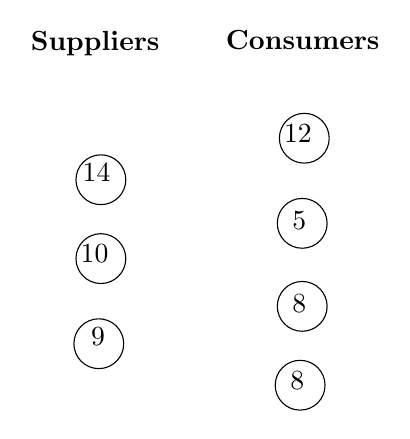
\begin{tikzpicture}[x=0.75pt,y=0.75pt,yscale=-1,xscale=1]
%uncomment if require: \path (0,209); %set diagram left start at 0, and has height of 209

%Shape: Circle [id:dp7908081224089281] 
\draw   (269,84) .. controls (269,77.37) and (274.37,72) .. (281,72) .. controls (287.63,72) and (293,77.37) .. (293,84) .. controls (293,90.63) and (287.63,96) .. (281,96) .. controls (274.37,96) and (269,90.63) .. (269,84) -- cycle ;
%Shape: Circle [id:dp1401138050936448] 
\draw   (269,122) .. controls (269,115.37) and (274.37,110) .. (281,110) .. controls (287.63,110) and (293,115.37) .. (293,122) .. controls (293,128.63) and (287.63,134) .. (281,134) .. controls (274.37,134) and (269,128.63) .. (269,122) -- cycle ;
%Shape: Circle [id:dp547936410525149] 
\draw   (268,163) .. controls (268,156.37) and (273.37,151) .. (280,151) .. controls (286.63,151) and (292,156.37) .. (292,163) .. controls (292,169.63) and (286.63,175) .. (280,175) .. controls (273.37,175) and (268,169.63) .. (268,163) -- cycle ;
%Shape: Circle [id:dp7958224490931569] 
\draw   (367,64) .. controls (367,57.37) and (372.37,52) .. (379,52) .. controls (385.63,52) and (391,57.37) .. (391,64) .. controls (391,70.63) and (385.63,76) .. (379,76) .. controls (372.37,76) and (367,70.63) .. (367,64) -- cycle ;
%Shape: Circle [id:dp24156316128200306] 
\draw   (366,105) .. controls (366,98.37) and (371.37,93) .. (378,93) .. controls (384.63,93) and (390,98.37) .. (390,105) .. controls (390,111.63) and (384.63,117) .. (378,117) .. controls (371.37,117) and (366,111.63) .. (366,105) -- cycle ;
%Shape: Circle [id:dp6344344926476859] 
\draw   (366,145) .. controls (366,138.37) and (371.37,133) .. (378,133) .. controls (384.63,133) and (390,138.37) .. (390,145) .. controls (390,151.63) and (384.63,157) .. (378,157) .. controls (371.37,157) and (366,151.63) .. (366,145) -- cycle ;
%Shape: Circle [id:dp2782911896772646] 
\draw   (365,183) .. controls (365,176.37) and (370.37,171) .. (377,171) .. controls (383.63,171) and (389,176.37) .. (389,183) .. controls (389,189.63) and (383.63,195) .. (377,195) .. controls (370.37,195) and (365,189.63) .. (365,183) -- cycle ;

% Text Node
\draw (271,75) node [anchor=north west][inner sep=0.75pt]   [align=left] {14};
% Text Node
\draw (270,114) node [anchor=north west][inner sep=0.75pt]   [align=left] {10};
% Text Node
\draw (275,154) node [anchor=north west][inner sep=0.75pt]   [align=left] {9};
% Text Node
\draw (368,56) node [anchor=north west][inner sep=0.75pt]   [align=left] {12};
% Text Node
\draw (372,98) node [anchor=north west][inner sep=0.75pt]   [align=left] {5};
% Text Node
\draw (372,138) node [anchor=north west][inner sep=0.75pt]   [align=left] {8};
% Text Node
\draw (371,175) node [anchor=north west][inner sep=0.75pt]   [align=left] {8};
% Text Node
\draw (246,11) node [anchor=north west][inner sep=0.75pt]   [align=left] {\textbf{Suppliers}};
% Text Node
\draw (340,11) node [anchor=north west][inner sep=0.75pt]   [align=left] {\textbf{Consumers}};


\end{tikzpicture}

The cost matrix for this problem is given to be \[
C=\begin{pmatrix} 5&3&4&6\\2&7&4&1 \\5&6&2&4 \end{pmatrix}
.\] We know that since $x_{ij}>0$ for all $i,j$ we have $\lambda_{i}+\mu_{j}=C_{ij}$. Solving these five equations gives us \[
\lambda_1 =0, \mu_1 =5, \mu_2 =3, \lambda_2 =4, \mu_3 =0, \lambda_3 =2, \mu_4 =2
.\] 
\begin{theorem}
	 Let $x$ be a basic feasible solution formed by the earlier process. Then the set of edges with strictly positive flow form a connected graph that has no cycle. This graph $T$ is a spanning tree with exactly $m+n-1$ edges.
\end{theorem}
\begin{proof}
	 The proof is beyond the scope of this course; we simply state this theorem, so that we know that this always happens!
\end{proof}
Now let's do the transport tableau as in the example. 
\[
\left|
	\begin{array}{c|c|c|c}
		\hline
		5 , 12 , 5 & 3,2, 3& 0,0, 4& 2,0,6\\
		\hline
		9,0,2&7,3,7&4,7,4&6,0,1\\
		\hline
		7,0,5&5,0,6&2,1,2&4,8,4\\
		\hline
	\end{array}
\right|
.\] 
If $c_{ij} \geq \lambda_{i}+\mu_{j}$ for all $i,j$ then $x$ is optimal. If $(i,j) \notin T$ such that $c_{ij}<\lambda_{i}+\mu_{j}$ then $(i,j)$ and the edges of $T$ of form a loop. Then we increase $x_{ij}$ until $x_{ab}=0$ for some $(a,b) \in T$. Then we update $\lambda, \mu$ and repeat until we get an optimal value. 
\subsubsection{Max flow - min cut}

\end{document}